\documentclass[a4paper]{article}

\usepackage[english]{babel}
\usepackage[utf8x]{inputenc}
\usepackage{amsmath}
\usepackage{graphicx}
\usepackage{hyperref}

\usepackage[colorinlistoftodos]{todonotes}
\usepackage[left=1in,right=1in]{geometry}
\title{CS 387 Database and Information Systems Lab\\
Project - ConsumerConnect}
\author{
Astha Agarwal (110050018)\\
Anmol Garg (110050020)\\
Deepali Adlakha (11D170020)}

\begin{document}
\maketitle


\section{Introduction - Application Domain}


As our CS 387 project, we have planned to make an online service portal, whereby people can interact with service providers and other customers to seek opinion and decide the appropriate service provider/service they want to use. Here, 'customers' refer to other users on the database, who also interact in a similar manner.\\On the other side, service providers will also be able to interact with users to know their potential customers. They can give details about the services they provide, and answer customer queries.\\The project involves crowdsourcing, search and social networking.\\


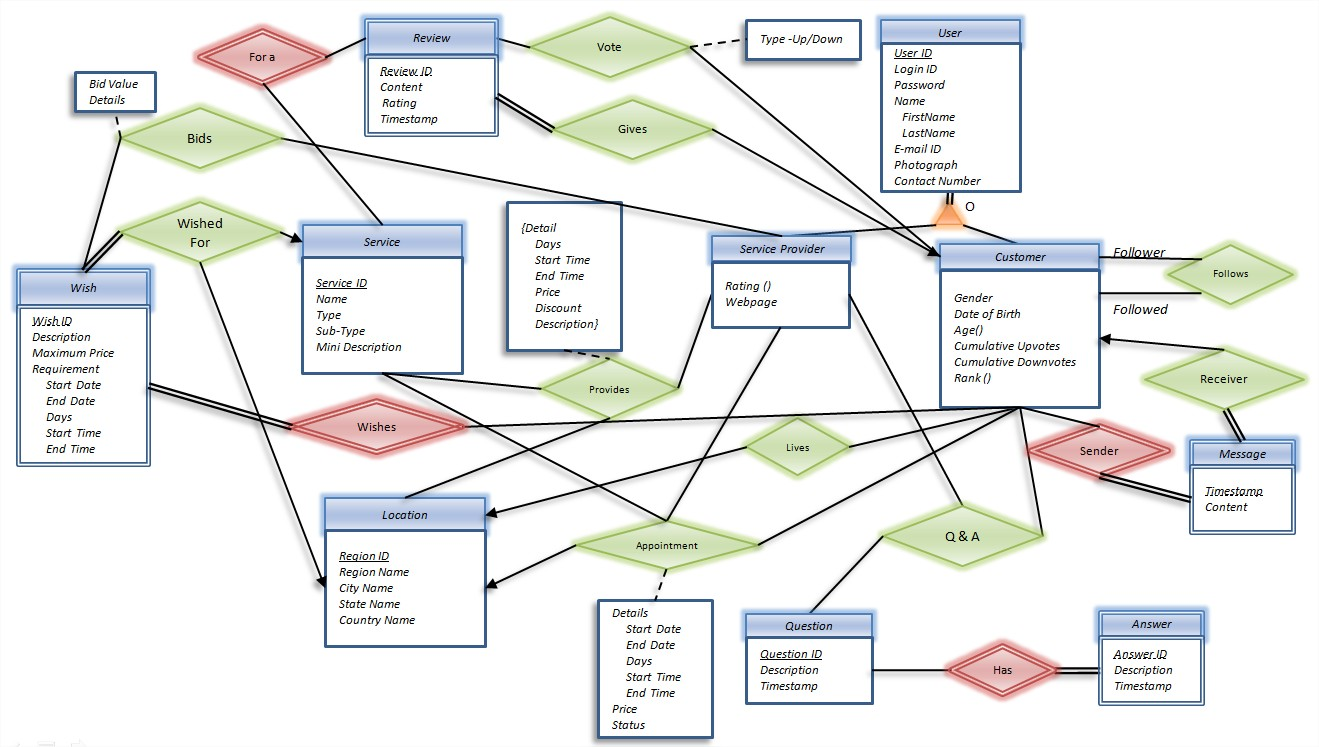
\includegraphics[width=160mm]{ermodel.jpg}



\section{Relational Model}


\subsection{For Entity Sets}
Assuming E/R Model Approach for hierarchy relationship in Users (Customer, ServiceProvider):

\begin{enumerate}

\item User(\underline{UserID}, LoginID, Password, FirstName, LastName, EmailID, Photograph, ContactNumber)

\item Customer(\underline{UserID}, Gender, DOB, CumulativeUpvotes, CumulativeDownvotes)

\item ServiceProvider(\underline{UserID}, Webpage)

\item Service(\underline{ServiceID}, Type, SubType, MiniDescription)

\item  \textbf{Many-to-Many Bad Relational Design -}\\  Review(\underline{ReviewID, ServiceID},CustomerUserID, Content, Rating, TimeStamp, \underline{VotedByCustomerUserID}, TypeOfVote)

\item Wish(\underline{WishID,CustomerUserID}, Description, MaximumPrice, StartDate, EndDate, Days, StartTime, EndTime, ServiceID, RegionID);

\item Question(\underline{QuestionID}, Description, TimeStamp);

\item Answer(\underline{QuestionID, AnswerID}, Description, TimeStamp);

\item Message(\underline {SenderCustomerUserID, Timestamp}, Content, ReceiverCustomerUserID)

\item \textbf{Many-to-One Bad Relational Design- } \\ Location(\underline{CustomerUserID, RegionID}, RegionName, CityName, StateName, CountryName) 
\end{enumerate}


\textbf{Note:} 
\begin{enumerate}
\item We have removed the CustomerID and ServiceProviderID, as they were redundant in providing unique identification to a type of user. In the E/R approach, we are anyway storing the UserID in Customer and ServiceProvider tables, and hence no need for another unique attribute.
\item We assume that there are no two end times for same start time, thus we haven't considered it as a primary key.
\item For the Many to Many relationship Votes from Review to Customer, we have added CustomerId as the attribute of Review, whereas there should be another relation relating Customer and Review for Votes. In this case, Review Information will be repeated and there can be an issue of consistency. 
\item For the Many to One relationship Lives from Customer to Street, we have added the CustomerID to Street as an attribute. This will not only lead to repetition of information and hence wastage of resources, but also create another problem. We have a ternary relation from ServiceProvider and Service to Street. \\Now we will have to map one location of a service given by a service provider to all tuples corresponding to every customer living at that location, which not only wastes space, but will also complicate search and other functions. So, in the relation for relationships, we have not considered this model, but the correct model which assumes that there is no CustomerID in Street table.

\end{enumerate}


For \textbf{OO Approach}, we have 3 relations again:

\begin{enumerate}
\item CustomerUser(UserID, LoginID, Password, Name, EmailID, Photograph, ContactNumber, Gender, DOB, CumulativePoints)
\item ServiceProviderUser(UserID, LoginID, Password, Name, EmailID, Photograph, ContactNumber, Webpage)
\item CustomerServiceProviderUser(UserID, LoginID, Password, Name, EmailID, Photograph, ContactNumber, Gender, DOB, CumulativePoints Webpage)

\end{enumerate}


\textbf{Note:} 
\begin{enumerate}

\item Here, there is no table for only User, because user has total participation in the "is a" relationship, and has at least one role as a Customer and/or a ServiceProvider. We note that in this case as well, separate CustomerID and ServiceProviderID are not required to distinguish entries. So, we have removed the two attributes from the relations.
\item Another point to note here is the problem associated with this structure. Suppose there is a User, who has only a customer profile. He starts offering a service and then he makes a service provider profile associated to the same account. In that case, we have to shift all his details from CustomerUser table to CustomerServiceProviderUser table. This might be a cumbersome task. Also, there is no authority that dictates that UserIDs cannot be same in the three tables.

\end{enumerate}


\subsection{For Relationship Sets}

\begin{enumerate}
\item Follows(\underline{FollowerCustomerUserID,FollowedCustomerUserID})
\item Bids(\underline{ServiceProviderUserID, WishID, CustomerUserID}, BidValue, Details)
\item Provides(\underline{ServiceProviderUserID, ServiceID, RegionID, Days, StartTime}, EndTime, Name, Price, Discount, Description)
\item Appointment(\underline{CustomerUserID, ServiceID, ServiceProviderUserID},\\ \underline{RegionID}, Price, Status, StartDate, EndDate, Days, StartTime, EndTime)  
\item QandA(\underline{CustomerUserID, ServiceProviderUserID, QuestionID})

\end{enumerate}




\subsection{Foreign Keys}
\begin{enumerate}
\item CustomerUserID and ServiceProviderUserId in any relation are foreign keys into UserID in Users.
\item ServiceID in any relation is foreign key into ServiceID in Services.
\item ReviewID in Experience is foreign key into ReviewID in Reviews.
\item WishID in Wishes, Bids and WishTime are foreign keys into WishID in Wish.
\item QuestionID in Answer is foreign key into QuestionID in Question.
\item QuestionID, AnswerID in QandA are foreign keys into QuestionID, AnswerID in Answer.
\item For location names, CountryName is a foreign key into Country, StateName is a foreign key into State and CityName is a foreign key into City.
\end{enumerate}



\subsection{Functional Dependencies}
\begin{enumerate}
\item As is obvious, all super keys determine the entire tuple.
\item In User relation: LoginID $\to$ (Password and other user details), EmailID $\to$ LoginID, Email-ID $\to$ UserID (In fact, LoginID and emailID are candidate keys.)
\item In the relation Location:  RegionName $\to$ RegionName, CityName, StateName, CountryName 
\item In the relation Reviews: (ReviewID, ServiceID) $\to$  CustomerUserID, Content, Rating, Timestamp
\item Functional dependencies for derived attributes (note that we have already removed them from the schema as the ER to Relational model design suggests.):
\begin{enumerate}
\item In the earlier relation Location attributes RegionName, CityName, StateName, CountryName are dependent only on RegionID which is a part of the key, hence a separate relation is formed corresponding to it.
\item In Customer relation: DOB $\to$ Age,  CumulativeUpvotes \& CumulativeDownvotes $\to$ Rank.
\end{enumerate}
\end{enumerate}

\subsection{Assertions}
\begin{enumerate}
\item In case of Appointments, the Start Time and the End Time should be ahead in the future (that is later than the Current time).
\item At the time of booking, the time for appointment should be subset of the time in Availability.
\item Rating should be between 0 to 5.
\item The timestamps in case of Questions, Answers and Reviews should be those of the past.
\item Discount should be between 0-100%.
\item Dates, days and months should be apt.
\item DOB should be of the past.
\item Contact No. should be of 10 digits.
\item Password should be of minimum 8 digits (includes one symbol, one number, one alphabet)
\item Vote type should be +1/-1. 
\item Gender should be Male/Female.
\end{enumerate}

\section{Normalisation}



\subsection{1NF}
\begin{enumerate}
\item The entity and relationship sets have already been normalised to 1NF form.
\item The components of composite attributes like Appointment Details have been flattened when converting to Relational Model.
\item The multivalued attribute like details of a service provided by service provider was stored separately as a table ProvidesDetails. However, in this case, there was no non-primary attribute in table Provides. So, we removed the table Provides and renamed ProvidesDetails as Provides, as it stores all the relevant information.

\end{enumerate}


\subsection{2NF}
\begin{enumerate}

\item User(\underline{UserID}, LoginID, Password, FirstName, LastName, EmailID, Photograph, ContactNumber)

\item Customer(\underline{UserID}, Gender, DOB, CumulativeUpvotes, CumulativeDownvotes)

\item ServiceProvider(\underline{UserID}, Webpage)

\item Service(\underline{ServiceID}, Type, SubType, MiniDescription)

\item In the earlier relation Reviews, attributes CustomerUserID, Content, Rating, Timestamp are dependent only on the subset of the candidate key that is (ReviewID, ServiceID), hence a separate relation corresponding to this is formed.
\subitem Review(\underline{ReviewID, ServiceID},CustomerUserID, Content, Rating, TimeStamp)
\subitem Vote(\underline{ReviewID, ServiceID, VotedByCustomerUserID}, TypeOfVote)

\item Wish(\underline{WishID,CustomerUserID}, Description, MaximumPrice, StartDate, EndDate, Days, StartTime, EndTime, ServiceID, RegionID);

\item Question(\underline{QuestionID}, Description, TimeStamp);

\item Answer(\underline{QuestionID, AnswerID}, Description, TimeStamp);

\item Message(\underline {SenderCustomerUserID, Timestamp}, Content, ReceiverCustomerUserID)

\item In the earlier relation Location attributes RegionName, CityName, StateName, CountryName are dependent only on RegionID which is a part of the key, hence a separate relation is formed corresponding to it.
\subitem Location(\underline{RegionID}, RegionName, CityName, StateName, CountryName)
\subitem Lives(\underline{RegionID, CustomerUserID})

\item Follows(\underline{FollowerCustomerUserID,FollowedCustomerUserID})
\item Bids(\underline{ServiceProviderUserID, WishID, CustomerUserID}, BidValue, Details)
\item Provides(\underline{ServiceProviderUserID, ServiceID, RegionID, Days, StartTime}, EndTime, Name, Price, Discount, Description)
\item Appointment(\underline{CustomerUserID, ServiceID, ServiceProviderUserID},\\ \underline{RegionID}, Price, Status, StartDate, EndDate, Days, StartTime, EndTime)  
\item QandA(\underline{CustomerUserID, ServiceProviderUserID, QuestionID})

\end{enumerate}


\subsection{BCNF and 3NF}
\begin{enumerate}
\item All the functional dependencies listed above have already been removed by 2NF normalisation.
\item The one non-trivial dependency which remains is the dependency in User Relation. However, we will not split up the relation for this because both LoginId and EmailID are taken as candidate keys.
\item Hence, we end up with a sufficiently normalised relation model that complies with BCNF anf 3NF rules.
\end{enumerate}



\end{document}